
\section{Custom Scenery Creation Work Flow}

The initial scene where buildings are to be created is, in this prototype, given.
If the architect was to generate a new starting scene, a work flow can be followed, as defined below.

\begin{figure}[!ht]
		\centering
		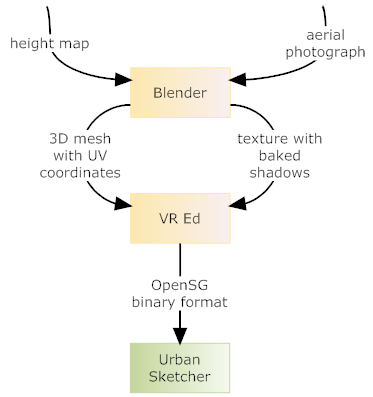
\includegraphics[width=7cm]{gfx/scene-work-flow.png}
		\caption{work flow to generate starting scene}
		\label{fig:scene-work-flow}
\end{figure}

Blender can apply a height map to a mesh, displacing its points.

If instead of a height map, the input data is in the form of of a topographic map
-- a set of contour lines defining places with the same altitude --
a Delaunay triangulation can be applied to the curves' points, generating a 3D mesh.
\TODO{DELAUNAY REF?}

The photograph can be edited prior to application so details can be omitted or enhanced.
Blender can then apply the photograph to the mesh.
The scene lighting can be positioned so it simulates different daylight conditions.
A new texture can then be generated by baking the shadows with the photograph.
Both the resulting texture and 3D mesh can be exported.

VR Ed \cite{VRED} is a 3D editor capable of importing several 3D data content and textures,
apply simple manipulations to them and save them in the OpenSG Binary format (OSB),
a format supported by our system.
One just has to import the Blender exported mesh (in a common format such as 3DS)
and save it to OSB.

%\TODO{blender, XML...}

\TODO{summary of implementation}
